\subsection{Introduction}
The theoretical foundation of Method 3 addresses the fundamental limitation of standard homography-based localization when perspective effects are insufficient. As demonstrated in the professor's slides, the standard homography-based method can fail with poor perspective, particularly when vanishing points are close to infinity, necessitating an iterative approach that can handle such degenerate cases.

\subsection{Theoretical framework}
\subsubsection{Geometric foundation and the poor perspective problem}
The core geometric insight behind this method is the reduction of the full 3D-to-2D projection problem to a simplified 2D-to-1D projection problem, involving a single unknown parameter: the rotation angle $\theta$ between the camera's $x$-axis and the direction of the vehicle's lateral axis (i.e., the direction of segment $AB$ or $CD$). Following the professor's methodology, rather than using the actual 3D points $E$, $A$, $B$, and $F$, the method considers vertically translated versions of these points whose $z$-coordinates match the $z$-coordinate of the camera center $O$, thus projecting them onto a horizontal plane through $O$.

\begin{figure}[h]
    \centering
    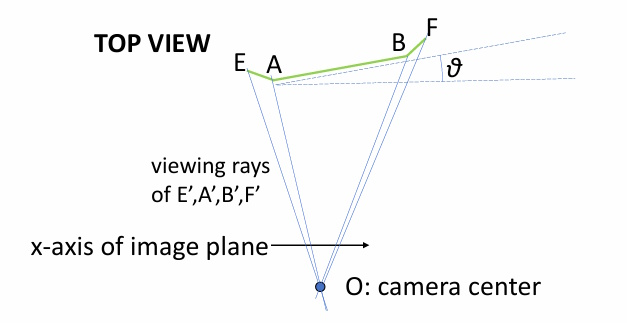
\includegraphics[width=0.6\textwidth]{Images/method3/schema.jpg}
    \caption{Top-view schematic showing camera center $O$, vehicle direction, and rotation angle $\theta$}
    \label{fig:theta_top_view}
\end{figure}

This transformation simplifies the projection model: since all model points now lie on a horizontal plane through the camera center, the problem reduces to estimating a 2D-to-1D projection governed by the single angle $\theta$, which can be recovered through geometric constraints.

\subsubsection{Iterative pose estimation framework}
The method employs an iterative refinement loop that alternates between enforcing geometric constraints and updating pose parameters. While individual geometric cues may be unreliable under poor perspective, their integration into a global iterative system yields a robust and solvable estimation framework.

\paragraph{Triangulation with known distances}
Given two image points with a known 3D separation, triangulation is used to recover their 3D positions. For points $A$ and $B$ with known distance $\texttt{AB\_distance}$ and estimated direction $\mathbf{u}_{AB}$, we solve:

\begin{equation}
    t \cdot \mathbf{r}_A - s \cdot \mathbf{r}_B = \texttt{AB\_distance} \cdot \mathbf{u}_{AB}
\end{equation}

where $\mathbf{r}_A$ and $\mathbf{r}_B$ are the normalized camera rays from back-projection, and $t$, $s$ are depth scalars.

\paragraph{Back-plane normal computation}
The orientation of the vehicle’s back plane is obtained from triangulated 3D points. For example, using points $A$, $B$, $C$, and $D$:

\begin{equation}
    \mathbf{n}_{\text{back}} = \texttt{normalize} \left( ( \mathbf{B}_{3d} - \mathbf{A}_{3d} ) \times ( \mathbf{D}_{3d} - \mathbf{C}_{3d} ) \right)
\end{equation}

\paragraph{Camera vertical direction}
The vertical direction of the camera is computed by rotating the back-plane normal $\mathbf{n}_{\text{back}}$ around the vehicle’s lateral axis $\mathbf{u}_{\text{dir}}$ by the known inclination angle $\phi$:

\begin{equation}
    \mathbf{v}_{\text{cam}} = \cos(\phi) \cdot \mathbf{n}_{\text{back}} + 
    \sin(\phi) \cdot ( \mathbf{u}_{\text{dir}} \times \mathbf{n}_{\text{back}} ) + 
    (1 - \cos(\phi)) \cdot \langle \mathbf{u}_{\text{dir}}, \mathbf{n}_{\text{back}} \rangle \cdot \mathbf{u}_{\text{dir}}
\end{equation}

\subsubsection{Horizon Line Projection and $\theta$ Computation}
A key step in the estimation pipeline involves projecting selected image points onto the horizon line to extract the yaw angle $\theta$.

\paragraph{Vertical Vanishing Point}
The vertical vanishing point $\mathbf{V}_z$ is computed from the camera's vertical direction:

\begin{equation}
    \mathbf{V}_z = \mathbf{K} \cdot \mathbf{v}_{\text{cam}}
\end{equation}

\paragraph{Horizontal Vanishing Line}
The horizon line $l_\infty$ is derived from the same vertical direction:

\begin{equation}
    l_\infty = \mathbf{K}^{-T} \cdot \mathbf{v}_{\text{cam}}
\end{equation}

\paragraph{Horizon Projection}
Each image point is projected onto the horizon by computing the intersection of the vertical line through $\mathbf{V}_z$ with $l_\infty$:

\begin{equation}
    \texttt{point\_on\_horizon} = (\mathbf{V}_z \times \mathbf{p}) \times l_\infty
\end{equation}

\paragraph{Yaw Angle Computation}
Once points $A''$ and $B''$ are projected on the horizon, the angle $\theta$ is extracted as:

\begin{equation}
    \theta = \arctan2( B''_y - A''_y, B''_x - A''_x )
\end{equation}

\subsubsection{Convergence and Stability}
The iterative algorithm converges by repeatedly satisfying the above constraints while adjusting the estimated angle and geometric parameters.

\subsection{Methodology}
\subsubsection{Initial Pose Estimation from Rear Plane Features}
The process begins with a coarse pose estimation using four coplanar points on the rear facade of the car—rear lights (A, B) and license plate corners (C, D). This estimate is based on vanishing point analysis: the lateral vanishing point $V_x$ is obtained from the intersection of the lines AB and CD and then back-projected using the camera matrix $K$ to obtain the lateral direction in 3D. Although this estimate is often inaccurate under poor perspective, it establishes a geometrically consistent initialization, including the back-plane normal and a first approximation of the camera’s vertical direction.

\subsubsection{Triangulation with Known Physical Constraints}
Once symmetric 2D points and their real-world distances are known from the vehicle CAD model, triangulation is used to reconstruct their 3D coordinates. The method back-projects the points to normalized rays and solves for depths that satisfy both the projection geometry and the known distance between points:

\begin{equation}
    t \cdot \mathbf{r}_A - s \cdot \mathbf{r}_B = \texttt{AB\_distance} \cdot \mathbf{u}_{AB}
\end{equation}

This constrained triangulation ensures physical plausibility and geometric consistency with the vehicle model even in the presence of poor perspective or noisy detections.

\subsubsection{Horizon Line Projection and Yaw Angle Computation}
The yaw angle $\theta$ is refined by projecting selected image points onto the horizon line. The vertical vanishing point $V_z$ is computed from the rotated back-plane normal using Rodrigues' formula. The horizontal vanishing line $l_\infty$ is then computed from $V_z$ and the calibration matrix $K$.

Each image point is projected onto $l_\infty$ by intersecting the vertical line through $V_z$ with the horizon line:

\begin{equation}
    \texttt{point}_{\text{horizon}} = (\mathbf{V}_z \times \mathbf{p}) \times l_\infty
\end{equation}

The yaw angle $\theta$ is then computed between projected points (e.g., $A''$, $B''$):

\begin{equation}
    \theta = \arctan2( B''_y - A''_y, B''_x - A''_x )
\end{equation}

When multiple symmetric pairs are available, a circular mean is used to robustly estimate the average yaw angle.

\subsubsection{Iterative Refinement Framework}
The core refinement loop performs the following updates at each iteration:

\begin{itemize}
    \item Update vehicle lateral direction (direction along $X$ axis) using the current $\theta$
    \item Perform triangulation using updated rays and known distances
    \item Refine the back-plane normal via cross product or SVD
    \item Rotate the back-plane normal to compute the new vertical direction
    \item Recompute vanishing geometry ($V_z$, $l_\infty$)
    \item Project symmetric points onto $l_\infty$ and update $\theta$
\end{itemize}

The updated yaw estimates are averaged using circular statistics. The loop continues until convergence criteria are met—either a small enough change in $\theta$, consistent geometry, or a max iteration count.

\subsection{Results and Evaluation}
The proposed method was evaluated on a test frame under poor perspective conditions, using the rear lights, license plate corners, and external rear lights (E–F) as symmetric features for pose estimation.

\subsubsection{Iterative Yaw Angle Convergence}
The method started from an initial yaw angle estimate of $\theta_{\text{init}} = 9.46^\circ$. Through the iterative refinement loop, the angle was progressively updated based on vanishing geometry and horizon line projections. The convergence log is as follows:

\begin{itemize}
    \item Iteration 1: $\theta = 6.27^\circ$, $\Delta\theta = -2.34^\circ$
    \item Iteration 2: $\theta = 5.89^\circ$, $\Delta\theta = -1.88^\circ$
    \item Iteration 3: $\theta = 5.58^\circ$, $\Delta\theta = -1.55^\circ$
    \item Iteration 4: $\theta = 4.37^\circ$, $\Delta\theta = -1.28^\circ$
    \item Iteration 5: $\theta = 4.17^\circ$, $\Delta\theta = -0.21^\circ$
    \item Iteration 6: $\theta = 4.14^\circ$, $\Delta\theta = -0.04^\circ$
\end{itemize}

The process converged after 7 iterations, yielding a final yaw estimate of $\theta_{\text{final}} = \mathbf{4.14^\circ}$. This demonstrates the effectiveness of the proposed method in refining vehicle orientation even under weak perspective cues.

\subsubsection{Geometric Consistency of Triangulated Features}

The method achieves high consistency between the triangulated 3D distances and the real-world measurements from the CAD model:

\begin{center}
    \begin{tabular}{lcc}
        \toprule
        \textbf{Feature Pair} & \textbf{Computed Distance (m)} & \textbf{Expected Distance (m)} \\
        \midrule
        A--B (rear lights, internal) & 0.860 & 0.86 \\
        C--D (license plate corners) & 0.520 & 0.52 \\
        E--F (rear lights, external) & 1.400 & 1.40 \\
        \bottomrule
    \end{tabular}
\end{center}

This confirms that the triangulation module, guided by the estimated yaw and direction vector, remains geometrically reliable.

\subsubsection{Final Projection Result}
Figure~\ref{fig:method3_result} shows the final result of the pose estimation: a 3D bounding box is projected onto the image using the computed pose and the simplified car model. The orientation aligns visually with the vehicle's position, confirming the correctness of the yaw and translation estimation.

\begin{figure}[h]
    \centering
    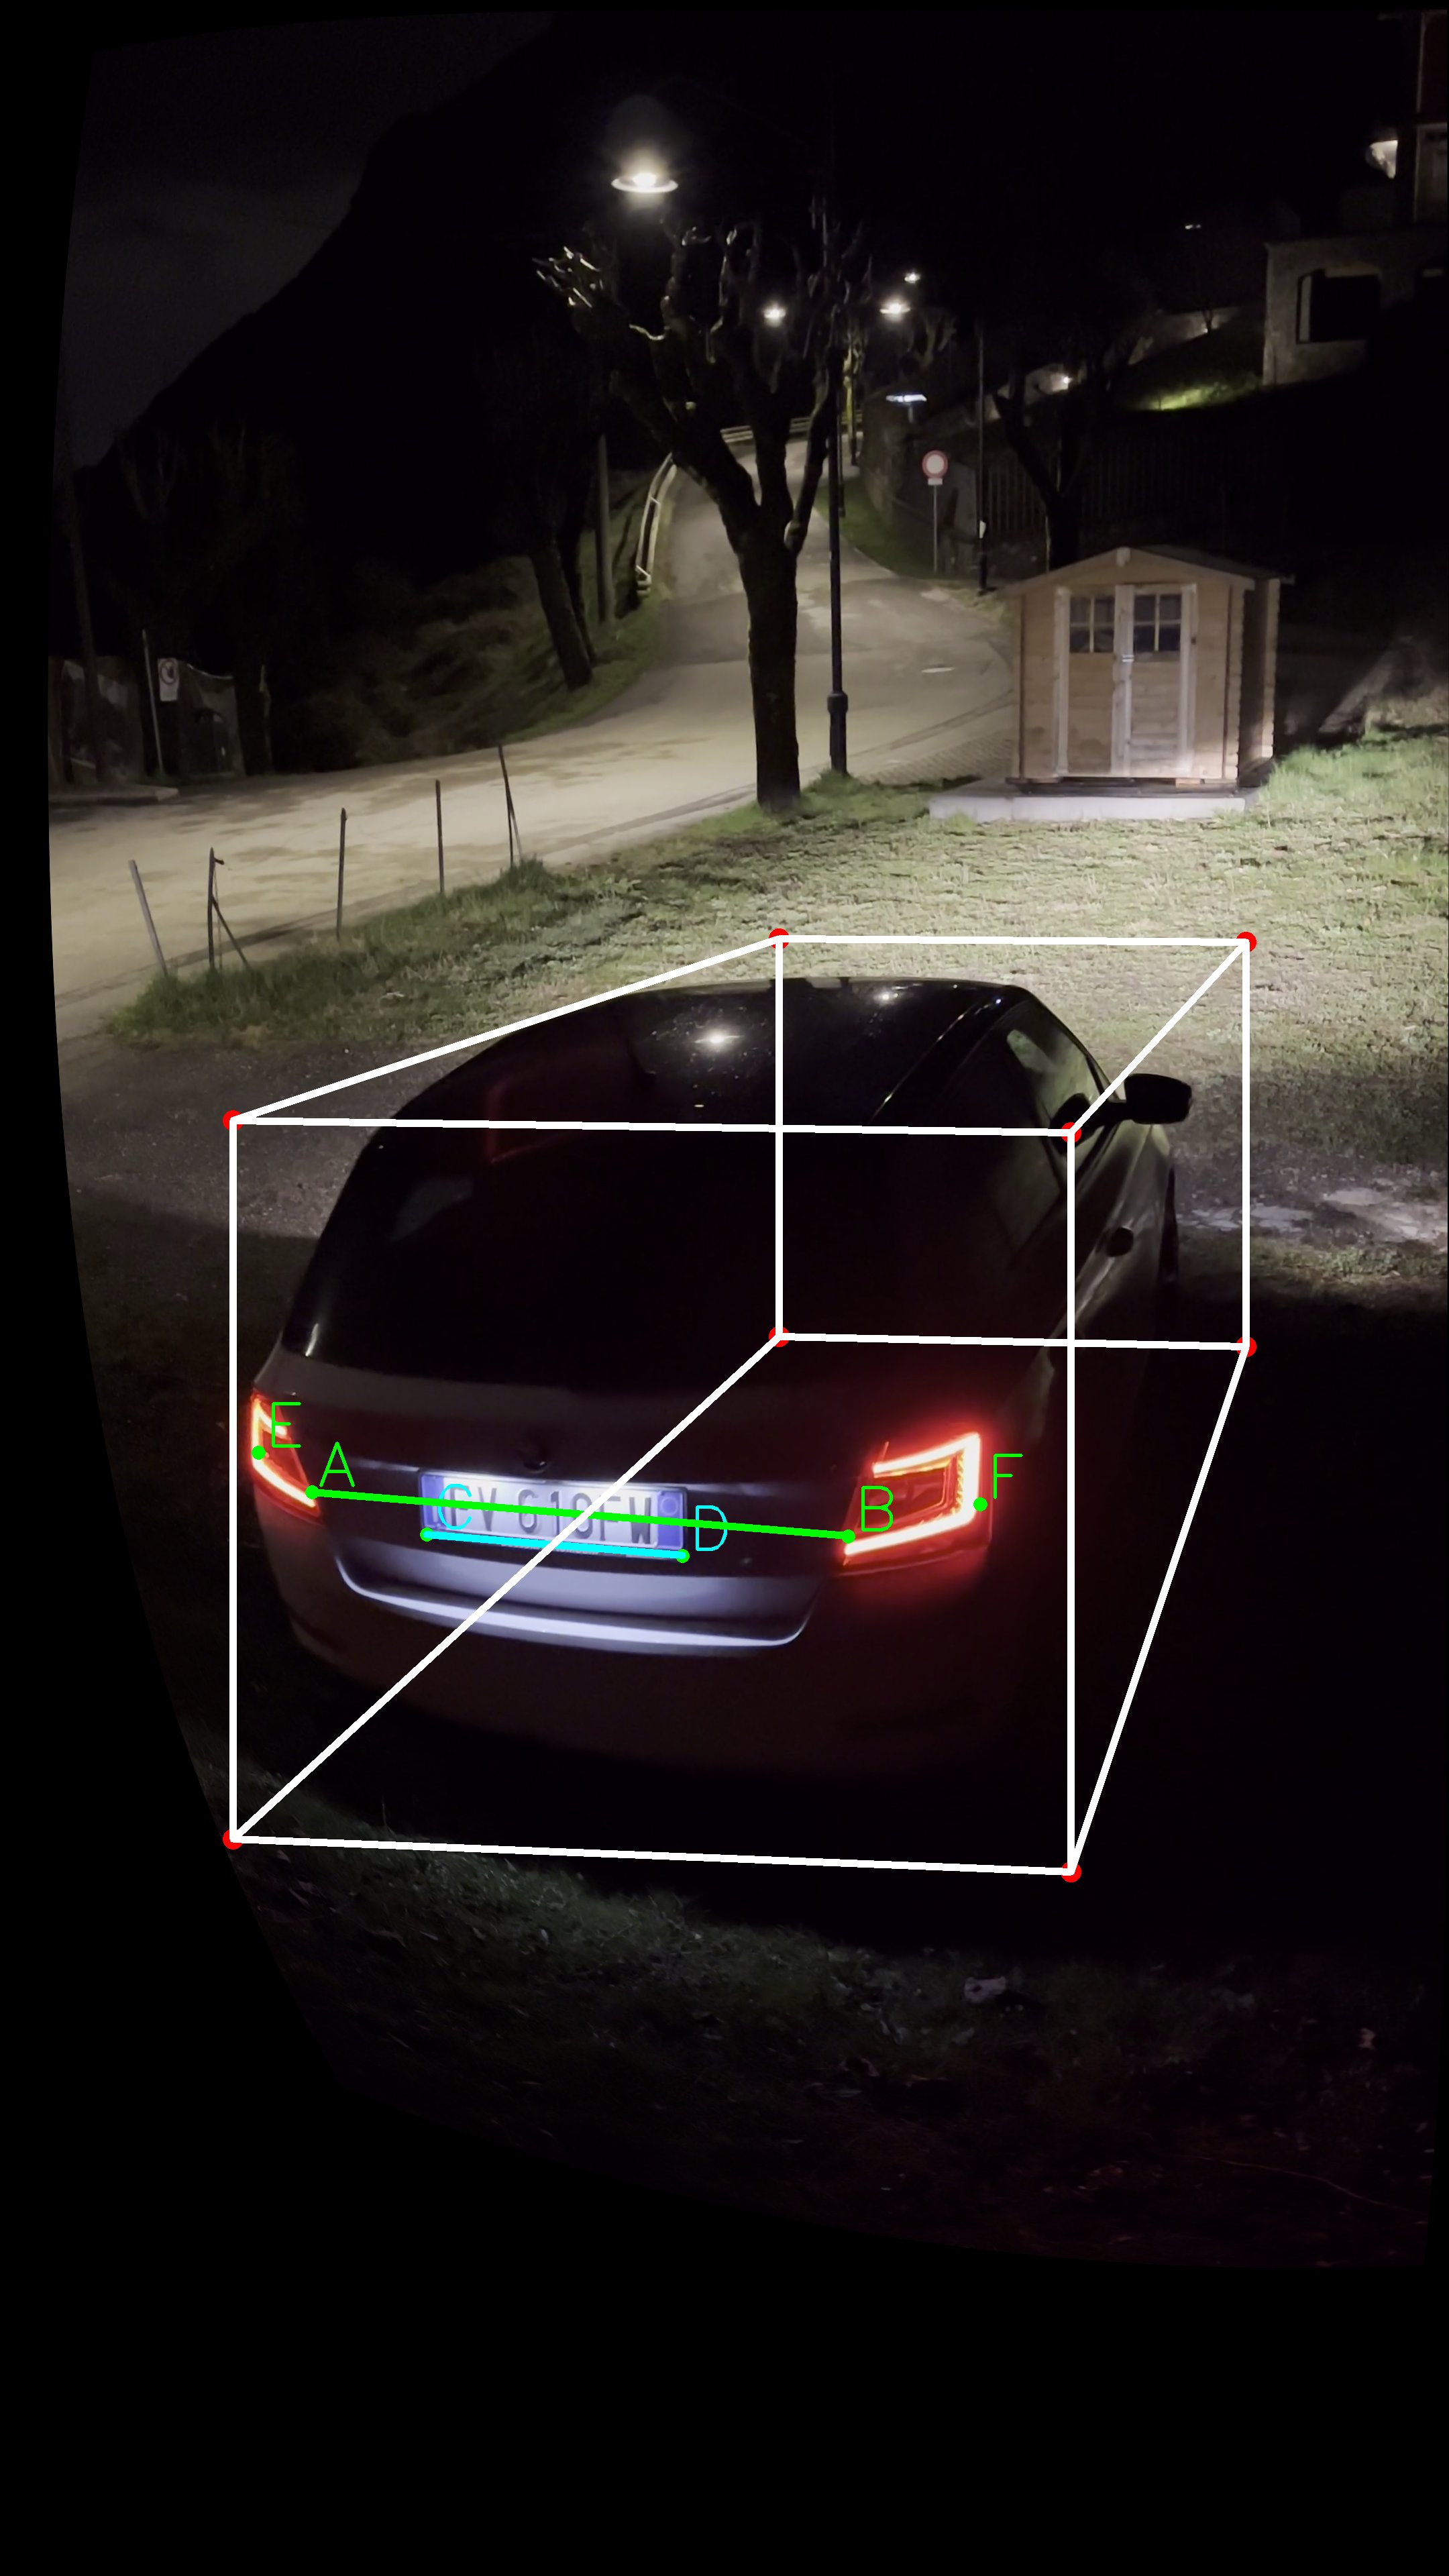
\includegraphics[width=0.35\textwidth]{Images/method3/final_bounding_box_method3.jpg}
    \caption{Final pose estimation result using Method 3. The bounding box aligns with the car's geometry, demonstrating successful localization under poor perspective.}
    \label{fig:method3_result}
\end{figure}